
\lecture{Inference With Independent Samples}{inference-testing-independent}
\section{Inference With Independent Samples}

\title{Inference With Two Samples}
\subtitle{Two Independent Samples}

%\author{Kelly Black}
%\institute{Clarkson University}
\date{10 November 2014}

\begin{frame}
  \titlepage
\end{frame}

\begin{frame}
  \frametitle{Outline}
  \tableofcontents[hideothersubsections,sectionstyle=show/hide]
\end{frame}



\subsection{Independent Samples}

\begin{frame}{Independent vs. Independent Samples}

  \begin{columns}[T]
    \column{.5\textwidth}
    Independent Samples

    \includegraphics[width=5cm]{img/independentSamples}

    \vfill
    \column{.5\textwidth}

    Dependent Samples

    \begin{tabular}{l@{$\Rightarrow$}r}
      ``Before'' & ``After'' \\ \hline
      $\textrm{before}_1$  & $\textrm{after}_1$ \\
      $\textrm{before}_2$  & $\textrm{after}_2$ \\
      $\textrm{before}_3$  & $\textrm{after}_3$ \\
      $\vdots$ & $\vdots$ \\
      $\textrm{before}_{\redText{N}}$ & $\textrm{after}_{\redText{N}}$  \\
    \end{tabular}


    \vfill

  \end{columns}

  
\end{frame}


\begin{frame}{Independent Samples}
  
  \vfill

  We cannot make a direct comparison between two random variables. In
  other words, $X-Y$ cannot refer to an individual test subject.

  \vfill

  We define 
  \begin{eqnarray*}
    W & = & X - Y.
  \end{eqnarray*}
  We assume that $X$ and $Y$ are independent random variables.

  \uncover<2->{%
    We get the following results:
    \begin{eqnarray*}
      W & = & X - Y, \\
      E[W] & = & \mu_x - \mu_y, \\
      \mathrm{Var}[X-Y] & = & \mathrm{Var}[X] + \mathrm{Var}[Y].
    \end{eqnarray*}
  }

  \vfill

\end{frame}


\begin{frame}{Comparing Two Groups}

  We have two populations and take some samples: \\
  \begin{columns}
    \column{.5\textwidth}
    \begin{tabular}{ll}
      Group 1 \\ \hline
      $x_1$  \\
      $x_2$  \\
      $x_3$  \\
      $\vdots$ \\
      $x_{\redText{N}}$  \\
    \end{tabular}

    \begin{eqnarray*}
      \bar{x} & = & \frac{x_1+x_2+\cdots+x_N}{N}
    \end{eqnarray*}

    \column{.5\textwidth}
    \begin{tabular}{ll}
      Group 2 \\ \hline
      $y_1$ \\
      $y_2$ \\
      $y_3$ \\
      ~ \\
      $\vdots$ \\
      ~ \\
      $y_{\redText{M}}$ \\
    \end{tabular}

    \begin{eqnarray*}
      \bar{y} & = & \frac{y_1+y_2+\cdots+y_M}{M}
    \end{eqnarray*}


  \end{columns}

  \vfill


  \vfill

\end{frame}


\begin{frame}{The Sample Distribution For the Difference}
  
    \begin{eqnarray*}
      E[\bar{x}-\bar{y}] & = & \mu_x - \mu_y, \\
      \mathrm{Var}[\bar{x}-\bar{y}] & = & \frac{\sigma^2_x}{N} + \frac{\sigma^2_y}{M}, \\
      \mathrm{Std.~Dev.}[\bar{x}-\bar{y}] & = & \sqrt{\frac{\sigma^2_x}{N} + \frac{\sigma^2_y}{M}}.
    \end{eqnarray*}

\end{frame}

\begin{frame}{Sample Standard Deviation}

  In practice we do not know the standard deviations and must rely on
  sample standard deviations.

    \begin{eqnarray*}
      s_w & = & \sqrt{\frac{s^2_x}{N} + \frac{s^2_y}{M}}, \\
      \mathrm{d.f.} & = & \frac{\lp \frac{s_x^2}{N} + \frac{s_y^2}{M}\rp^2}{
          \frac{s_x^4}{N^2(N-1)} + \frac{s_y^4}{M^2(M-1)}},
    \end{eqnarray*}
    and you round \redText{down} for the number of degrees of
    freedom. Note that there is a simpler alternative calculation for
    the number of degrees of freedom, df=$\min(N,M)-1$.
  
  
\end{frame}

\subsection{Examples}

\begin{frame}
  \frametitle{Clicker Quiz}%

  \iftoggle{clicker}{%

    The optical clarity of two polishing techniques are
    compared. Fifteen samples from method one gives a sample mean of
    98.5\% total transmittance with a sample standard deviation of
    2.0\% transmittance. Seventeen samples from method two gives a
    sample mean of 97.3\% transmittance with a sample standard
    deviation of 1.5\% transmittance. Does the second method give a
    lower transmittance?


    \vfill

    What is the hypothesis test?
    \begin{tabular}{l@{\hspace{3em}}l}
      A: & $H_0:~\mu_1-\mu_2=0$, $H_a:~\mu_1-\mu_2\neq 0$  \\
      B: & $H_0:~\mu_1-\mu_2=0$, $H_a:~\mu_1-\mu_2> 0$  \\
      C: & $H_0:~\mu_1-\mu_2=0$, $H_a:~\mu_1-\mu_2< 0$  \\
      D: & $H_0:~\mu_1-\mu_2 < 0$, $H_a:~\mu_1-\mu_2 = 0$  \\
    \end{tabular}

    \vfill
    \vfill
    \vfill
  }

\end{frame}


\begin{frame}
  \frametitle{Example}

  The optical clarity of two polishing techniques are
  compared. Fifteen samples from method one gives a sample mean of
  98.5\% total transmittance with a sample standard deviation of 2.0\%
  transmittance. Seventeen samples from method two gives a sample mean
  of 97.3\% transmittance with a sample standard deviation of 1.5\%
  transmittance. Does the second method give a lower transmittance?

    \vfill
    
    \only<2->{%
      We have sufficient evidence to reject $H_0$ at the 5\%
      significance level using a $t$-distribution with twenty-five
      degrees of freedom.  }
\end{frame}

\begin{frame}{By the way...}

\redText{Note:}
The method used in the previous example assumes that the variances are
different. 

\vfill

\redText{Problem:} 
There are times when you assume the null hypothesis is correct you
\blueText{do not} want to assume that the variances are 
different!


\vfill
\vfill
  
\end{frame}

\begin{frame}{Pooled Variance}

  \redText{Sometimes} you do not want to assume that the distributions
  are different. In these cases you should \redText{pool} the data,
  \begin{eqnarray*}
    s_p^2 & = & \frac{(n-1)s_x^2 + (m-1)s_y^2}{n+m-2},
  \end{eqnarray*}
  and the standard deviation of $\bar{x}-\bar{y}$ is 
  \begin{eqnarray*}
    s & = & s_p \sqrt{\frac{1}{n}+\frac{1}{m}},
  \end{eqnarray*}
  and we use $n+m-2$ degrees of freedom.
  
\end{frame}

\begin{frame}
  \frametitle{Clicker Quiz}%

  \iftoggle{clicker}{%

    There are two methods of producing a compound, and we want to
    compare how much power is required in the two processes. In method
    one twelve samples and taken, and a sample mean of 1,200KW with a
    standard deviation of 180KW is found for the power
    requirements. For method two fifteen samples yield a sample mean
    of 1,300KW with a sample standard deviation of 190KW. Assuming
    that the variance of the methods are the same does the second
    method require more energy?

    \vfill

    What is the hypothesis test?
    \begin{tabular}{l@{\hspace{3em}}l}
      A: & $H_0:~\mu_1-\mu_2=0$, $H_a:~\mu_1-\mu_2\neq 0$  \\
      B: & $H_0:~\mu_1-\mu_2=0$, $H_a:~\mu_1-\mu_2> 0$  \\
      C: & $H_0:~\mu_1-\mu_2=0$, $H_a:~\mu_1-\mu_2< 0$  \\
      D: & $H_0:~\mu_1-\mu_2 < 0$, $H_a:~\mu_1-\mu_2 = 0$  \\
    \end{tabular}

    \vfill
    \vfill
    \vfill
  }

\end{frame}


\begin{frame}{Example}

  There are two methods of producing a compound, and we want to
  compare how much power is required in the two processes.  In method
  one twelve samples and taken, and a sample mean of 1,200KW with a
  standard deviation of 180KW is found for the power requirements. For
  method two fifteen samples yield a sample mean of 1,300KW with a
  sample standard deviation of 190KW. Assuming that the variance of
  the methods are the same does the second method require more energy?

  \vfill

  \only<2->{%
    We do not have sufficient evidence to reject $H_0$ at the 5\%
    significance level assuming a $t$-distribution with twenty-five
    degrees of freedom \redText{and a pooled variance}.  }
\end{frame}


\begin{frame}{Example}

  Two methods to coat a metal are compared. In the first method ten
  samples are taken and the sample mean for the thickness is 0.32mm
  with a sample standard deviation of 0.08mm. In the second method
  twelve samples are taken giving a sample mean of 0.35mm and a sample
  standard deviation of 0.12mm. Determine the 95\% confidence interval
  for the difference.

  \vfill

  \only<2->{%

    The 95\% confidence interval is from -.12mm and .06mm  assuming a $t$-distribution with
    nineteen degrees of freedom.
    
  }
\end{frame}

\begin{frame}
  \frametitle{Clicker Quiz}%

  \iftoggle{clicker}{%

    Two designs are to be tested. In design one eleven samples are
    taken, and the sample mean for the temperature of the heat sink is
    187C with a sample standard deviation of 14C. In design two nine
    samples are taken with a sample mean of 192C and a sample standard
    deviation of 12C. Determine if there is a difference using a 95\%
    confidence level. Use a pooled variance.

    \vfill

    What is the hypothesis test?
    \begin{tabular}{l@{\hspace{3em}}l}
      A: & $H_0:~\mu_1-\mu_2=0$, $H_a:~\mu_1-\mu_2\neq 0$  \\
      B: & $H_0:~\mu_1-\mu_2=0$, $H_a:~\mu_1-\mu_2> 0$  \\
      C: & $H_0:~\mu_1-\mu_2=0$, $H_a:~\mu_1-\mu_2< 0$  \\
      D: & $H_0:~\mu_1-\mu_2 < 0$, $H_a:~\mu_1-\mu_2 = 0$  \\
    \end{tabular}

    \vfill
    \vfill
    \vfill
  }

\end{frame}



\begin{frame}{Example}

  Two designs are to be tested. In design one eleven samples are
  taken, and the sample mean for the temperature of the heat sink is
  187C with a sample standard deviation of 14C. In design two nine
  samples are taken with a sample mean of 192C and a sample standard
  deviation of 12C. Determine if there is a difference using a 95\%
  confidence level. Use a pooled variance.

  \vfill

  \only<2->{%
    We do not have sufficient evidence to reject $H_0$ at the 5\%
    significance level assuming a $t$-distribution with eighteen
    degrees of freedom.  }
\end{frame}


% LocalWords:  Clarkson pausesection hideallsubsections
